\section{Experiments}

\begin{figure*}[t]
\begin{center}
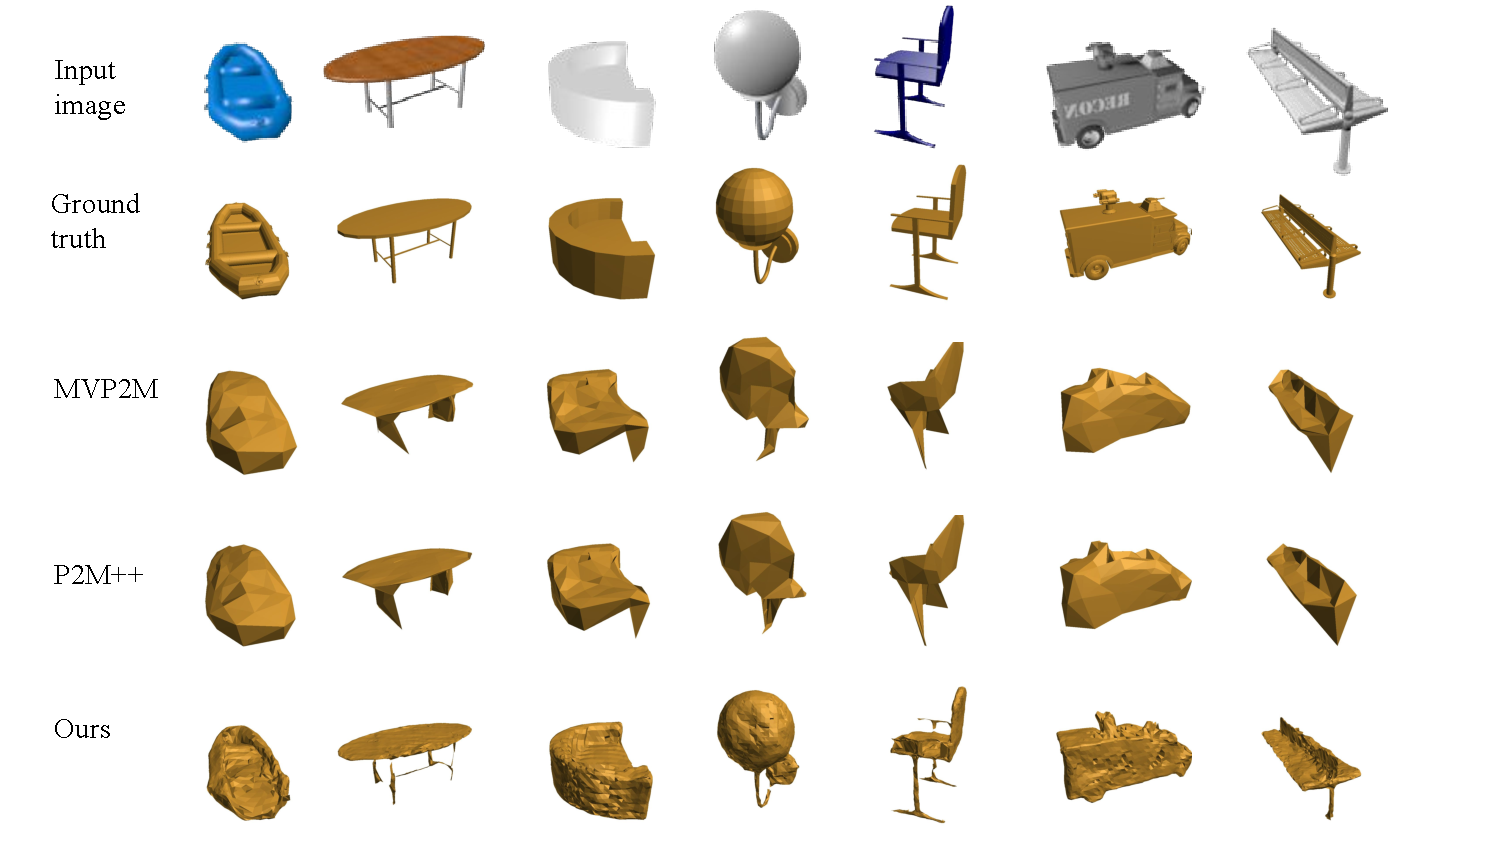
\includegraphics[width=\linewidth]{imgs/qualitative_evaluation.pdf}
\end{center}
\vspace{-4mm}
\caption{
    \textbf{Qualitative evaluation} on ShapeNet dataset. \textbf{From top to bottom}: one of the input images, ground truth mesh, multi-view extended Pixel2Mesh, Pixel2Mesh++, and ours.
    Our predictions are closer to the actual shape, especially for the objects with more complex topologies.}

    % Two of three input images used by all the systems are shown along with a pair of camera views of the predictions.
    % The quality of shapes generated by our method is consistently better.
    % Note that in the last input of category \emph{Watercraft} the baselines generate shapes closer to \emph{Car} while our predictions are much closer to the actual shape.
% }
\vspace{-4mm}
\label{fig:qualitative_evaluation}
\end{figure*}

\subsection{Experimental Setup}
\label{subsec:experimental_setup}

\paragraph{Comparisons}
We evaluate the proposed method against various multi-view shape generation methods.
The state-of-the-art method is Pixel2Mesh++~\cite{wen2019pixel2mesh++} (referred as \emph{P2M++}). \cite{wen2019pixel2mesh++} also provide a baseline by directly extending Pixel2Mesh~\cite{wang2018pixel2mesh} to operate on multi-view images (referred as \emph{MVP2M}) using their statistical feature pooling method to aggregate features from multiple color images.
% This implementation is closer to \emph{Ours-P2M} system design in that it predicts the output mesh by series for GCN deformations
% starting from an initial ellipsoid without having a fairly accurate initial object mesh.
% Also, \emph{Ours-P2M} uses the same architecture for the mesh deformations as \emph{MVP2M}. Hence, the changes in performance can be directly attributed to our depth based features, added geometric constraints and attentive feature pooling.
Results from additional multi-view shape generation baselines 3D-R2N2~\cite{3dr2n2} and LSM~\cite{kar2017lsm} are also reported.
\vspace{-4mm}
\paragraph{Dataset}
We evaluate our method against the state-of-the-art methods on the dataset from~\cite{3dr2n2}
which is a subset of ShapeNet~\cite{chang2015shapenet} and has been widely used by recent 3D shape generation methods.
It contains 50K 3D CAD models from 13 categories.
Each model is rendered with a transparent background from 24 randomly chosen camera viewpoints to obtain color images.
The corresponding camera intrinsics and extrinsics are provided in the dataset.
Since the dataset does not contain depth images, we render them using a custom depth renderer at the same viewpoints as the color images and with the same camera intrinsics.
We follow the training/testing/validation split of~\cite{gkioxari2019meshrcnn}.
\vspace{-4mm}
\paragraph{Implementation}
% We train the proposed model using the same settings as Pixel2Mesh++ and MVP2M for fair comparison.
% The same 3 views from each model are used as input and the images are resized to a resolution of 224$\times$224 for feature extraction/depth prediction.
For the depth prediction module, we follow the original MVSNet~\cite{yao2018mvsnet} implementation.
The output depth dimensions reduces by a factor of 4 to 56$\times$56 from the 224$\times$224 input image.
The number of depth hypotheses is chosen as 48 which offers a balance between accuracy and running/training time efficiency.
These depth hypotheses represent values from $0.1$ m to $1.3$ m at an interval of $25$ mm.
These values were chosen based on the range of depths present in the dataset.
% The final cost volume is of dimensions 56$\times$56$\times$48 which is regularized using a 3D convolutional network.

The hierarchical features obtained from "Contrastive Depth Features Extractor" are of total 4800 dimensions for each view.
The aggregated multi-view features are compressed to 480 dimensional after applying attentive feature pooling.
5 attention heads are used for merging multi-view features.
The loss function weights are set as $\lambda_{\text{chamfer}}=1$, $\lambda_{\text{normal}}=1.6\times10^{-4}$, $\lambda_{\text{depth}}=0.1$, $\lambda_{\text{contrastive}}=0.001$ and $\lambda_{\text{voxel}}=1$.
Two settings of $\lambda_{\text{edge}}$ were used, $\lambda_{\text{edge}}=0$ (referred as \emph{Best}) which gives better quantitative results and $\lambda_{\text{edge}}=0.2$ (referred as \emph{Pretty}) which gives better qualitative results.

% Ours models are implemented in PyTorch deep learning framework using open-source Pixel2Mesh/Mesh R-CNN implementation.
\vspace{-4mm}
\paragraph{Training and Runtime}
The network is optimized using Adam optimizer with a learning rate of $10^{-4}$.
The training is done on 5 Nvidia RTX-2080 GPUs with effective batch size 5.
% The number of GPUs and batch size were chosen in order to maximize training speed while staying within the GPU memory limit.
The depth prediction network (MVSNet) is trained independently for 30 epochs.
Then the whole system is trained for another 40 epochs with the weights of the MVSNet frozen.
Our system is implemented in PyTorch deep learning framework and it takes around 60 hours for training.

% The initial learning rate is set to 1e-4 which is reduced to 1e-5 after 30 epochs and 1e-6 after 45 epochs.
% \emph{Ours-P2M} takes around 100 hours to train while \emph{Ours-MRCNN} takes around 50 hours.
% This training time is similar to Pixel2Mesh++.
\vspace{-4mm}
\paragraph{Evaluation Metric}
Following~\cite{wang2018pixel2mesh, wen2019pixel2mesh++}, we use F1-score as our evaluation metric.
The F1-score is the harmonic mean of precision and recall where the precision/recall are calculated by finding the percentage of points in the predicted/ground truth that can find a nearest neighbor from the other within a threshold.
We provide evaluations with two threshold values: $\tau$ and $2\tau$ where $\tau=10^{-4}$  m$^2$.
% (in terms of squared Euclidean distance).
% The output meshes can vary in number of vertices but are re-sampled to 6466 points before evaluating the F1-score~\cite{wang2018pixel2mesh, wen2019pixel2mesh++}. \rakesh{might not be true}
\vspace{-2mm}
\subsection{Comparison with previous Multi-view Shape Generation Methods}
We quantitatively compare our method against previous works for multi-view shape generation in~\tableref{baseline_comparison} and show the effectiveness of our methods in improving the shape quality. Our method outperforms the state-of-the-art method  Pixel2Mesh++~\cite{wen2019pixel2mesh++} with
a decrease in chamfer distance to ground truth by 34\% and 15\% increase in F1-score at threshold $\tau$.
Note that in~\tableref{baseline_comparison} the same model is trained for all the categories but accuracy on individual categories as well as average over the categories are evaluated.
We provide the chamfer distances in the appendix.
\begin{table}[ht]
\begin{center}
\resizebox{\linewidth}{!}{
\begin{tabular}{|c|cccccc|cccccc|}
    \hline
    \multirow{3}{*}{Category}&
    \multicolumn{6}{c|}{F-score ($\tau$) $\uparrow$}&
    \multicolumn{6}{c|}{F-score ($2\tau$) $\uparrow$}\\
    & \multirow{2}{*}{3D-R2N2}  & \multirow{2}{*}{LSM}  & \multirow{2}{*}{MVP2M}    & \multirow{2}{*}{P2M++} & Ours & \bf{Ours}
    & \multirow{2}{*}{3D-R2N2}  & \multirow{2}{*}{LSM}  & \multirow{2}{*}{MVP2M}    & \multirow{2}{*}{P2M++} & Ours & \bf{Ours} \\
    &                           &                       &                           &                        & (pretty) & \bf{(best)} &
                                &                       &                           &                        & (pretty) & \bf{(best)} \\
    \hline
    Couch       & 45.47 & 43.02 & 53.17 & 57.56 & 71.63 & \bf{73.63}    & 59.97 & 55.49 & 73.24 & 75.33 & 85.28 & \bf{88.24} \\
    Cabinet     & 54.08 & 50.80 & 56.85 & 65.72 & 75.91 & \bf{76.39}    & 64.42 & 60.72 & 76.58 & 81.57 & 87.61 & \bf{88.84} \\
    Bench       & 44.56 & 49.33 & 60.37 & 66.24 & 81.11 & \bf{83.76}    & 62.47 & 65.92 & 75.69 & 79.67 & 90.56 & \bf{92.57} \\
    Chair       & 37.62 & 48.55 & 54.19 & 62.05 & 77.63 & \bf{78.69}    & 54.26 & 64.95 & 72.36 & 77.68 & 88.24 & \bf{90.02} \\
    Monitor     & 36.33 & 43.65 & 53.41 & 60.00 & 74.14 & \bf{76.64}    & 48.65 & 56.33 & 70.63 & 75.42 & 86.04 & \bf{88.89} \\
    Firearm     & 55.72 & 56.14 & 79.67 & 80.74 & 92.92 & \bf{94.32}    & 76.79 & 73.89 & 89.08 & 89.29 & 96.81 & \bf{97.67} \\
    Speaker     & 41.48 & 45.21 & 48.90 & 54.88 & 66.02 & \bf{67.83}    & 52.29 & 56.65 & 68.29 & 71.46 & 79.76 & \bf{82.34} \\
    Lamp        & 32.25 & 45.58 & 50.82 & 62.56 & 72.47 & \bf{75.93}    & 49.38 & 64.76 & 65.72 & 74.00 & 82.00 & \bf{85.33} \\
    Cellphone   & 58.09 & 60.11 & 66.07 & 74.36 & 85.57 & \bf{86.45}    & 69.66 & 71.39 & 82.31 & 86.16 & 93.40 & \bf{94.28} \\
    Plane       & 47.81 & 55.60 & 75.16 & 76.79 & 89.23 & \bf{92.13}    & 70.49 & 76.39 & 86.38 & 86.62 & 94.65 & \bf{96.57} \\
    Table       & 48.78 & 48.61 & 65.95 & 71.89 & 82.37 & \bf{83.68}    & 62.67 & 62.22 & 79.96 & 84.19 & 90.24 & \bf{91.97} \\
    Car         & 59.86 & 51.91 & 67.27 & 68.45 & 77.01 & \bf{80.43}    & 78.31 & 68.20 & 84.64 & 85.19 & 88.99 & \bf{92.33} \\
    Watercraft  & 40.72 & 47.96 & 61.85 & 62.99 & 75.52 & \bf{80.48}    & 63.59 & 66.95 & 77.49 & 77.32 & 86.77 & \bf{90.35} \\
    \hline
    Mean        & 46.37 & 49.73 & 61.05 & 66.48 & 78.58 & \bf{80.80}    & 62.53 & 64.91 & 77.10 & 80.30 & 88.49 & \bf{90.72} \\
    \hline
\end{tabular}}
\end{center}
\vspace{-4mm}
\caption{
    \textbf{Qualitative comparison} against state-of-the-art multi-view shape generation methods. We report F-score on each semantic category along with the mean over all categories using two thresholds $\tau$ and $2\tau$ for nearest neighbor match where ${\tau}$=$10^{-4}$ m$^2$.
}
\label{table:baseline_comparison}
\end{table}


\vspace{-2mm}
We also provide visual results for qualitative assessment of the generated shapes by our \emph{Pretty} model in~\figref{qualitative_evaluation} which shows that it is able to more accurately predict topologically diverse shapes.

% ~\tableref{baseline_comparison} show the ablation study
% performed to quantify the improvements from different aspects of our methods.
% Our methods outperform all the baselines in all the semantic categories.
% \figref{qualitative_evaluation} shows the qualitative comparison between the shapes generated by the different methods.
% The baseline methods suffer from various artifacts and discontinuities while ours generate shapes with higher fidelity.
\vspace{-2mm}
\subsection{Ablation studies}
% Extensive ablation studies are performed to quantify the contributions of each component.
% The "stats pooling" baseline is obtained by replacing the attention-based feature pooling with statistical features from Pixel2Mesh++.
% Similarly, "simple attention" baseline is obtained by replacing our feature pooling with feature fusion technique proposed in~\cite{hu2019randla,yang2020robust} where the pooled features are weighted sum of the multi-view features.
% We can see that our rendered depth loss, contrastive depth input and attention-based feature pooling individually improve the accuracy of the predicted mesh.
\vspace{-2mm}
\paragraph{Contrastive Depth Feature Extraction}
We evaluate several methods for contrastive feature extraction (\subsecref{contrastive_depth_feature_extraction}). These methods are
1) \emph{Input Concatenation}: using the concatenated rendered and predicted depth maps as input to the VGG feature extractor,
2) \emph{Input Difference}: using the difference of the two depth maps as input to VGG,
3) \emph{Feature Concatenation}: concatenating features from rendered and predicted depths extracted by shared VGG,
4) \emph{Feature Difference}: using difference of the features from the two depth maps extracted by shared VGG, and
5) \emph{Predicted depth only}: using the VGG features from the predicted depths only.
6) \emph{Rendered depth only}: using the VGG features from the rendered depths only.
The quantitative results are summarized in Table~\ref{table:contrastive_feature_extraction} and shows that \emph{Input Concatenation} method produces better results than other formulations.
% remains more details depth information and our Contrastive Depth Feature Extraction is able to encode the difference between the predicted depth map and rendered depth map from each deformation stage.

\begin{table}[ht]
% \captionsetup{font=footnotesize,labelfont=footnotesize}
\begin{center}
\footnotesize
\begin{tabular}{ l c c }
\toprule[1pt]
 &F1-$\tau$ &F1-2$\tau$ \\ \hline
(1) Input Concatenation \qquad \qquad  \qquad  \qquad  \qquad  & \textbf{80.80} & \textbf{90.72} \\
(2) Input Difference & 80.41 & 90.54 \\
(3) Feature Concatenation   & 80.45 & 90.54 \\
(4) Feature Difference & 80.30 & 90.40 \\
(5) Predicted Depth only & 79.40 & 89.95 \\
(6) Rendered Depth only & 78.20 & 88.90 \\
\bottomrule[1pt]
\end{tabular}
\end{center}
\vspace{-4mm}
\caption{\textbf{Comparisons of different contrastive depth formulations}. In 1st and 2nd rows, concatenation and difference of the rendered and predicted depths are fed to VGG feature extractor while in 3rd and 4th rows, concatenation and difference of the VGG features from the depths is used for mesh refinement. 5 uses VGG features from predicted depths only while 6 uses VGG features from rendered depths only. \siyu{``Input Concatenation'' and ``Input Difference'' are hard to understand. Change them to another expression, such as ``Depth image concatenation''.}}
\label{table:contrastive_feature_extraction}
\end{table}



\vspace{-4mm}
\paragraph{Accuracy with different settings}
\tableref{ablation_study} shows the contribution of different components towards the final accuracy. Naively extending the single-view Mesh R-CNN~\cite{gkioxari2019meshrcnn} to multiple views using statistical feature pooling~\cite{wen2019pixel2mesh++} for mesh refinement (row 1) gives an F1-score of 72.74\% for threshold $\tau$ which is 6.26\% improvement over Pixel2Mesh++.
We further extend the above method with our probabilistic multi-view voxel grid prediction in row 2 and get a 4.23\% improvement.

In row 3 of~\tableref{ablation_study} we use our contrastive depth features instead of RGB features for mesh refinement and get 2.7\% improvement.
We then replace the statistical feature pooling with the proposed attention method and get 0.19\% improvement.
The improvement is not significant on our final architecture but we found the multi-head attention to perform better on more light-weight architectures.
We also evaluate the effect of using additional regularization from contrastive depth losses: rendered depth vs predicted depth in the 5th rows of which improves the score by 0.98\%.
In row 6 we use ground truth instead of predicted depths on our final model which gives the upper bound on our mesh prediction accuracy in relation to the depth prediction accuracy as 84.58\%.

% \vspace{-4mm}
% \paragraph{Sphere initialization}
% Row 8 uses a sphere as the coarse shape instead of cubified voxel grid.

% \begin{table}[ht]
% \begin{center}
% \resizebox{\linewidth}{!}{
% \begin{tabular}{|c|c|c|c|c|c|c|}
%     \hline
%     Metric & Ours-P2M & - rendered depth loss & - contrastive depth & stats pooling & simple attention & GT-depth \\
%     \hline
%     F1-$\tau$ & TBD & TBD & TBD & TBD & TBD & \textbf{TBD} \\
%     F1-$2\tau$ & TBD & TBD & TBD & TBD & TBD & \textbf{TBD} \\
%     % Chamfer distance (mm) & 0.30 & 0.33 & 0.33 & 0.325 & 0.30 & \textbf{0.18} \\
%     \hline
% \end{tabular}}
% \end{center}
% \caption{
%     Ablation Study. ${\tau}$=$10^{-4}$ m$^2$
% }
% \label{table:ablation_study_p2m}
% \end{table}

\begin{table}[ht]
% \captionsetup{font=footnotesize,labelfont=footnotesize}
\begin{center}
\footnotesize
\begin{tabular}{ l c c }
\toprule[1pt]
 &F1-$\tau$ &F1-2$\tau$   \\ \hline
(1) Naive multi-view Mesh R-CNN \qquad \qquad  \qquad  \qquad  \qquad & 72.74 & 84.99 \\
(2) + Multi-view voxel grid prediction & 76.97 & 88.24 \\
(3) + Contrastive depth input             & 79.63 & 90.10 \\
(4) + Multi-head attention pooling   & 79.82    & 90.18  \\
(5) \bf{+ Contrastive depth loss (final model)}  & \textbf{80.80} & \textbf{90.72}\\
% (6) Baseline + rendered vs GT depth loss    & 80.35 & 90.55 \\
% (7) Baseline + rendered vs predicted depth loss + rendered vs GT depth loss    & 80.45 & 90.56 \\
% (8) Baseline with simple attention          & 80.03 & 90.21 \\
(6) Using GT depth (final model)                 & \textbf{84.58} & \textbf{92.86} \\
% (10) Sphere initialization                  & 73.78 & 85.49 \\
\bottomrule[1pt]
\end{tabular}
\end{center}
\vspace{-4mm}
\caption{
    \textbf{Comparison of shape generation accuracy with different settings} of additional contrastive depth losses, multi-view feature pooling.
    The Baseline framework uses multi-head attention mechanism without any contrastive depth losses.
    \siyu{Remove (2) Multi-head attention pooling and (6) Using GT depth (final model). Both statistics seem to be irrelevant to the paper.}
}
\label{table:ablation_study}
\end{table}

% \begin{table}[t]
% % \captionsetup{font=footnotesize,labelfont=footnotesize}
% \begin{center}
% \footnotesize
% \begin{tabular}{ l c c }
% \toprule[1pt]
%  &F1-$\tau$ &F1-2$\tau$ \\ \hline
% With Perceptual Feature Loss \qquad \qquad  \qquad  \qquad  \qquad  & 74.87 & 86.92 \\
% Without Perceptual Feature Loss & 75.30 & 87.12 \\
% \bottomrule[1pt]
% \end{tabular}
% \end{center}
% \caption{Comparisons of different contrastive depth formulations, where \emph{Pred} indicates predicted depth map from MVSNet, \emph{Rend} indicates rendered depth map from deformed mesh model, $\ominus$ means element-wise minus, $\otimes$ means concatenation. In 1 and 2 concatenation and difference of the depths are fed to VGG feature extractor while in 3 and 4 concatenation and difference of the VGG features from the depths is used for mesh refinement \rakesh{Note: These results will be updated with the results from our final architecture}}
% \label{table:perceptual_loss}
% \end{table}



% using the difference
% Instead of using contrastive depth input i.e. concatenated predicted and rendered depths
% (refer to~\figref{system_architecture})
% we directly use a single channeled predicted depth as input. Column 4 of
% \tableref{ablation_study} and \tableref{ablation_study_mrcnn} show the results of these experiments.

% % \begin{table}[ht]
% \begin{center}
% \footnotesize
% \begin{tabular}{c | c c c c c c}
%     \hline
%     Metric & RGB-Ours & Depth-Ours & RGBD-Ours & RGB 1-view & Depth 1-view & RGBD 1-view \\
%     \hline
%     F1-$\tau$   & 31.27 & 30.30 & 31.61 & 25.19 & 23.78 & 26.06 \\
%     F1-$2\tau$  & 44.46 & 43.16 & 44.86 & 36.75 & 35.14 & 37.74 \\
%     \hline
% \end{tabular}
% \end{center}
% \caption{
%     Accuracy of predicted voxel of individual views against probabilistically merged multi-view voxel grids, where the first three columns indicate the accuracy of multi-view voxel generations while the last three columns show single-view. The voxel branch was trained separately without the mesh refinement. Evaluation is conducted after cubify and the depth maps are generated from MVSNet.
% }
% \label{table:multiview_voxel_accuracy}
% \end{table}
\begin{table}[ht]
\noindent \scriptsize \footnotesize
\begin{minipage}[t]{0.5\textwidth}
\centering
\begin{tabular}{c | c c}
    \hline
    Metric      & Single-view & Multi-view \\
    \hline
    F1-$\tau$   & 25.19 & 31.27 \\
    F1-$2\tau$  & 36.75 & 44.46 \\
    \hline
\end{tabular}
\caption{
    \textbf{Accuracy of predicted voxel grids} from single-view prediction compared against the proposed probabilistically merged multi-view voxel grids. The voxel branch was trained separately without the mesh refinement and evaluation was performed on the cubified voxel grids. We use three views for probabilistic grid merging.
}
\label{table:multiview_voxel_accuracy}
\end{minipage}
\hspace{0.1cm}
\noindent \scriptsize \footnotesize
\begin{minipage}[t]{0.5\textwidth}
\centering
\begin{tabular}{c | c c c c}
    \hline
    Metric & Cubified & Stage-1 & Stage-2 & Stage-3 \\
    \hline
    F1-$\tau$   & 31.48 & 76.78 & 79.88 & 80.80  \\
    F1-$2\tau$  & 44.40 & 88.32 & 90.19 & 90.72  \\
    \hline
\end{tabular}
\caption{
    \textbf{Accuracy of the refined meshes at different GCN stages}. 1, 2 and 3 indicate the performance at the corresponding graph convolution blocks while \emph{Cubified} is for the cubified voxel grids used as input for the first GCN block. All the stages, including the voxel prediction, were trained jointly and hence the accuracy of voxel predictions varies from that in~\tableref{multiview_voxel_accuracy}.
}
\label{table:gcn_stages}
\end{minipage}
\end{table}



% \paragraph{Different Input Modalities}
% We analyze the accuracy of using different input modalities (RGB vs Depth vs RGB-D) for the voxel branch and mesh branch (GCN refinement) in~\tableref{input_modality_accuracy}.

% \begin{table}[ht]
\begin{center}
\footnotesize
\begin{tabular}{c c | c c}
\toprule[1pt]
    Voxel branch    & Mesh branch   & F1-$\tau$         & F1-$2\tau$ \\ \hline
    RGB             & RGB           & 79.66             & 89.98 \\
    Depth           & Depth         & 77.07             & 88.20 \\
    RGB-D           & RGB           & 78.42             & 89.32 \\
    RGB             & RGB-D         & \textbf{80.80}    & \textbf{90.55} \\
    % RGB-D         & RGBD-D        & \textbf{81.15}    & \textbf{90.92}
\bottomrule[1pt]
\end{tabular}
\end{center}
\caption{
    Accuracy with different input modalities of voxel and mesh.
    % \rakesh{More extensive combinations of input modalities can be performed if needed}
    % Using RGB-D for both voxel and mesh branch gave the best results with the most recent architecture
    % but all the other ablation study experiments were performed with RGB+RGB-D, so we are not reporting RGBD+RGBD to avoid confusion
}
\label{table:input_modality_accuracy}
\end{table}


\vspace{-4mm}
\paragraph{Number of View}
We test the performance of our framework with respect to the number of views.
\tableref{number_of_input_views} shows that the accuracy of our method increases as we increase the number of input views for training.
These experiments also validate that the attention-based feature pooling can efficiently encode features from different views to take advantage of larger number of views.

\tableref{number_of_test_views} shows the results when using different number of views during testing on our model trained with 3 views
which indicates that increasing the number of views during testing does not improve the accuracy while decreasing the number of views can cause a significant drop in accuracy.
% The accuracy is very close to the corresponding models trained with higher number of views indicating our model can learn with fewer number of views and generalize to a larger number.
% -> \rakesh{this conclusion is not true, training with larger number of views gets significantly better performance}
\begin{table}[ht]
\noindent \scriptsize \footnotesize
\begin{minipage}[t]{0.5\textwidth}
\centering
\begin{tabular}{ l | c c c c c }
    \hline
    Metric & 2 & 3 & 4 & 5 & 6\\
    \hline
    F1-$\tau$  & 73.60 & 80.80 & 82.61 & 83.76 & 84.25 \\
    F1-$2\tau$ & 85.80 & 90.72 & 91.78 & 92.73 & 93.14 \\
    \hline
\end{tabular}
\caption{
    \textbf{Accuracy w.r.t the number of views during training}.
    The evaluation was performed on the same number of views as training.
    % The evaluation was performed on the same number of views (3 views) for a fair comparison. \rakesh{Not true}
}
\label{table:number_of_input_views}
\end{minipage}
\hspace{0.1cm}
\noindent \scriptsize \footnotesize
\begin{minipage}[t]{0.5\textwidth}
\centering
\begin{tabular}{ l | c c c c c }
    \hline
    Metric & 2 & 3 & 4 & 5 & 6 \\
    \hline
    F1-$\tau$   & 72.46 & 80.80 & 80.98 & 80.94 & 80.85 \\
    F1-$2\tau$  & 84.49 & 90.72 & 91.03 & 91.16 & 91.20 \\
    \hline
\end{tabular}
\caption{
    \textbf{Accuracy w.r.t the number of views during testing}.
    The same model trained with 3 views was used in all of the cases.
}
\label{table:number_of_test_views}
\end{minipage}
\vspace{-4mm}
\end{table}
\vspace{-4mm}

